% Options for packages loaded elsewhere
% Options for packages loaded elsewhere
\PassOptionsToPackage{unicode}{hyperref}
\PassOptionsToPackage{hyphens}{url}
%
\documentclass[
  ignorenonframetext,
]{beamer}
\newif\ifbibliography
\usepackage{pgfpages}
\setbeamertemplate{caption}[numbered]
\setbeamertemplate{caption label separator}{: }
\setbeamercolor{caption name}{fg=normal text.fg}
\beamertemplatenavigationsymbolsempty
% remove section numbering
\setbeamertemplate{part page}{
  \centering
  \begin{beamercolorbox}[sep=16pt,center]{part title}
    \usebeamerfont{part title}\insertpart\par
  \end{beamercolorbox}
}
\setbeamertemplate{section page}{
  \centering
  \begin{beamercolorbox}[sep=12pt,center]{section title}
    \usebeamerfont{section title}\insertsection\par
  \end{beamercolorbox}
}
\setbeamertemplate{subsection page}{
  \centering
  \begin{beamercolorbox}[sep=8pt,center]{subsection title}
    \usebeamerfont{subsection title}\insertsubsection\par
  \end{beamercolorbox}
}
% Prevent slide breaks in the middle of a paragraph
\widowpenalties 1 10000
\raggedbottom
\AtBeginPart{
  \frame{\partpage}
}
\AtBeginSection{
  \ifbibliography
  \else
    \frame{\sectionpage}
  \fi
}
\AtBeginSubsection{
  \frame{\subsectionpage}
}
\usepackage{iftex}
\ifPDFTeX
  \usepackage[T1]{fontenc}
  \usepackage[utf8]{inputenc}
  \usepackage{textcomp} % provide euro and other symbols
\else % if luatex or xetex
  \usepackage{unicode-math} % this also loads fontspec
  \defaultfontfeatures{Scale=MatchLowercase}
  \defaultfontfeatures[\rmfamily]{Ligatures=TeX,Scale=1}
\fi
\usepackage{lmodern}

\usetheme[]{metropolis}
\ifPDFTeX\else
  % xetex/luatex font selection
  \setmathfont[]{Latin Modern Math}
\fi
% Use upquote if available, for straight quotes in verbatim environments
\IfFileExists{upquote.sty}{\usepackage{upquote}}{}
\IfFileExists{microtype.sty}{% use microtype if available
  \usepackage[]{microtype}
  \UseMicrotypeSet[protrusion]{basicmath} % disable protrusion for tt fonts
}{}
\makeatletter
\@ifundefined{KOMAClassName}{% if non-KOMA class
  \IfFileExists{parskip.sty}{%
    \usepackage{parskip}
  }{% else
    \setlength{\parindent}{0pt}
    \setlength{\parskip}{6pt plus 2pt minus 1pt}}
}{% if KOMA class
  \KOMAoptions{parskip=half}}
\makeatother


\usepackage{longtable,booktabs,array}
\usepackage{calc} % for calculating minipage widths
\usepackage{caption}
% Make caption package work with longtable
\makeatletter
\def\fnum@table{\tablename~\thetable}
\makeatother
\usepackage{graphicx}
\makeatletter
\newsavebox\pandoc@box
\newcommand*\pandocbounded[1]{% scales image to fit in text height/width
  \sbox\pandoc@box{#1}%
  \Gscale@div\@tempa{\textheight}{\dimexpr\ht\pandoc@box+\dp\pandoc@box\relax}%
  \Gscale@div\@tempb{\linewidth}{\wd\pandoc@box}%
  \ifdim\@tempb\p@<\@tempa\p@\let\@tempa\@tempb\fi% select the smaller of both
  \ifdim\@tempa\p@<\p@\scalebox{\@tempa}{\usebox\pandoc@box}%
  \else\usebox{\pandoc@box}%
  \fi%
}
% Set default figure placement to htbp
\def\fps@figure{htbp}
\makeatother

\ifLuaTeX
  \usepackage{luacolor}
  \usepackage[soul]{lua-ul}
\else
  \usepackage{soul}
  \makeatletter
  \let\HL\hl
  \renewcommand\hl{% fix for beamer highlighting
    \let\set@color\beamerorig@set@color
    \let\reset@color\beamerorig@reset@color
    \HL}
  \makeatother
\fi




\setlength{\emergencystretch}{3em} % prevent overfull lines

\providecommand{\tightlist}{%
  \setlength{\itemsep}{0pt}\setlength{\parskip}{0pt}}



 


\setbeamerfont{title}{size=\large}
\makeatletter
\@ifpackageloaded{caption}{}{\usepackage{caption}}
\AtBeginDocument{%
\ifdefined\contentsname
  \renewcommand*\contentsname{Table of contents}
\else
  \newcommand\contentsname{Table of contents}
\fi
\ifdefined\listfigurename
  \renewcommand*\listfigurename{List of Figures}
\else
  \newcommand\listfigurename{List of Figures}
\fi
\ifdefined\listtablename
  \renewcommand*\listtablename{List of Tables}
\else
  \newcommand\listtablename{List of Tables}
\fi
\ifdefined\figurename
  \renewcommand*\figurename{Figure}
\else
  \newcommand\figurename{Figure}
\fi
\ifdefined\tablename
  \renewcommand*\tablename{Table}
\else
  \newcommand\tablename{Table}
\fi
}
\@ifpackageloaded{float}{}{\usepackage{float}}
\floatstyle{ruled}
\@ifundefined{c@chapter}{\newfloat{codelisting}{h}{lop}}{\newfloat{codelisting}{h}{lop}[chapter]}
\floatname{codelisting}{Listing}
\newcommand*\listoflistings{\listof{codelisting}{List of Listings}}
\makeatother
\makeatletter
\makeatother
\makeatletter
\@ifpackageloaded{caption}{}{\usepackage{caption}}
\@ifpackageloaded{subcaption}{}{\usepackage{subcaption}}
\makeatother

\usepackage{bookmark}
\IfFileExists{xurl.sty}{\usepackage{xurl}}{} % add URL line breaks if available
\urlstyle{same}
\hypersetup{
  pdfauthor={Giorgio Arcara},
  hidelinks,
  pdfcreator={LaTeX via pandoc}}


\author{Giorgio Arcara}
\date{}

\begin{document}


\begin{frame}
% TITLE SLIDES
\title{Metodi Statistici per la Neuropsicologia Forense\\ \vspace{1em} \emph{2. La cornice teorica}}
\author{Giorgio Arcara,\\ Università di Padova \\ IRCCS San Camillo, Venezia}

\titlegraphic{

\vspace*{7cm}

\includegraphics[scale=0.15]{Figures/LogoSanCamilloIRCCS_Unipd_alpha.png}
\hfill 
\includegraphics[scale=0.15]{Figures/CC_license_3_0.png}
}
\maketitle
\end{frame}

\begin{frame}{Misurazione}
\phantomsection\label{misurazione}
\emph{``We may say that measurement, in the broadest sense, is defined
as the assignment of numerals to objects or event, according to
rules.''}

\emph{Stevens (1946)} \pause \vspace{2em}

Questa è stata una definizione estremamente popolare che tuttora domina
la neuropsicologia
\end{frame}

\begin{frame}{Una definizione di misurazione da filosofia e fisica}
\phantomsection\label{una-definizione-di-misurazione-da-filosofia-e-fisica}
Non si misurano oggetti ma \emph{proprietà} di oggetti:

``Sia \(O\) un certo insieme di oggetti caratterizzati dall'avere la
proprietà P e sia \(\mathbb{R}\) l'insieme dei numeri Reali i quali
possono essere ordinati in accordo al criterio ``essere maggiore o
uguale a'', si definisce misurazione:

Chiamiamo \(O_p\) l'insieme di oggetti tali che si crei un
``omomorfismo'' tra \((O_p, \succcurlyeq)\) e \((\mathbb{R}, \geq)\).

Dove \(\succcurlyeq\) indicano \emph{relazioni d’ordine empirico}
(oggetti fisici) e \(\geq\) \emph{relazioni d’ordine numerico}''

\begin{flushright}
\emph{Boniolo e Vidali, Filosofia della scienza, p. 321}
\end{flushright}
\end{frame}

\begin{frame}{Limiti della definizione di Stevens}
\phantomsection\label{limiti-della-definizione-di-stevens}
\begin{columns}
  \begin{column}{0.5\textwidth}
    \begin{figure}
    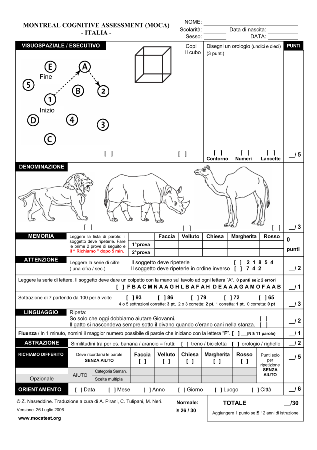
\includegraphics[scale=0.5]{Figures/MOCA.png}
    \end{figure}
  \end{column}
  \begin{column}{0.5\textwidth}
    \textbf{Esaminiamo il MoCa:}
    \pause
    \vspace{2em}
    
    Cosa notate nei punteggi delle parti che lo compongono?
    
    \vspace{2em}
    Cosa notate nei compiti?
  \end{column}
\end{columns}
\end{frame}

\begin{frame}{Limiti della definizione di Stevens}
\phantomsection\label{limiti-della-definizione-di-stevens-1}
Supponiamo di avere un tavolo che sia lungo 40 cm, mentre un'altro
tavolo è lungo 20 cm. Concludereste che il tavolo è lungo il doppio
dell'altro? \pause \vspace{2em} Supponiamo ad un test di memoria una
persona ottiene 40, mentre un'altra 20. Vi sentireste di concludere che
quella persona ha il doppio della memoria dell'altra. \pause
\vspace{2em} Spesso la misurazione in psicologia/neuropsicologia non
rispetta alcuni principi di misurazioni più rigide (es. fisica)
\end{frame}

\begin{frame}{Oggettività}
\phantomsection\label{oggettivituxe0}
Un concetto che emerge spesso quando si parla di misurazione, di test,
di statistica è quello di oggettività. \pause \vspace{2em} I test
infatti vengo spesso considerati più ``oggettivi''. Vale la pena quindi
approfondire questo concetto \pause \vspace{2em} Definiamo qui
oggettività come una proprietà che si applica ad una valutazione, ad un
test, o come \emph{l'indipedenza dell'esaminatore dal risultato}
\end{frame}

\begin{frame}{Oggettività}
\phantomsection\label{oggettivituxe0-1}
\footnotesize``L'esame neuropsicologico forense viene spesso considerato
un esame oggettivo del funzionamento cognitivo. In un'ideale gerarchia
delle sorgenti d'evidenza, tale esame si collocherebbe molto più in alto
rispetto alle evidenze cliniche più o meno sofisticate (self-reports,
informant-based reports, interviste cliniche, rating scales, ecc.), e
dovrebbe pertanto essere ``promosso'' a rango più elevato (al pari degli
esami biochimici, radiologici, ecc.). Dopo che il clinico ha esaminato
il soggetto e ha formulato le sua ipotesi preliminari, chiede agli esami
strumentali di confermarle, confutarle o correggerle attraverso dati
oggettivi, indipendenti sia dal giudizio dell'esaminatore e dalle sue
distorsioni, sia da ogni variabile estranea all'oggetto d'indagine, in
particolare dalle contaminazioni dovute alla soggettività
dell'esaminato.''

\begin{flushright}
\emph{Copia verbatim da  Stracciari, Bianchi, Sartori (2010); Neuropsicologia Forense}
\end{flushright}

Il concetto di oggettività verrà ripreso più avanti, specie con
\emph{inter-rater agreement}
\end{frame}

\begin{frame}{Cosa sono i test}
\phantomsection\label{cosa-sono-i-test}
``Un test è una \textbf{procedura sistematica} per
\textbf{l’osservazione del comportamento} di una persona e per la sua
\textbf{descrizione con l’aiuto di una scala numerica} o un sistema di
categorie''

\begin{flushright}
  \emph{(Cronbach, 1990, p.32)}
\end{flushright}
\pause

\begin{flushright}
  \begin{figure}
    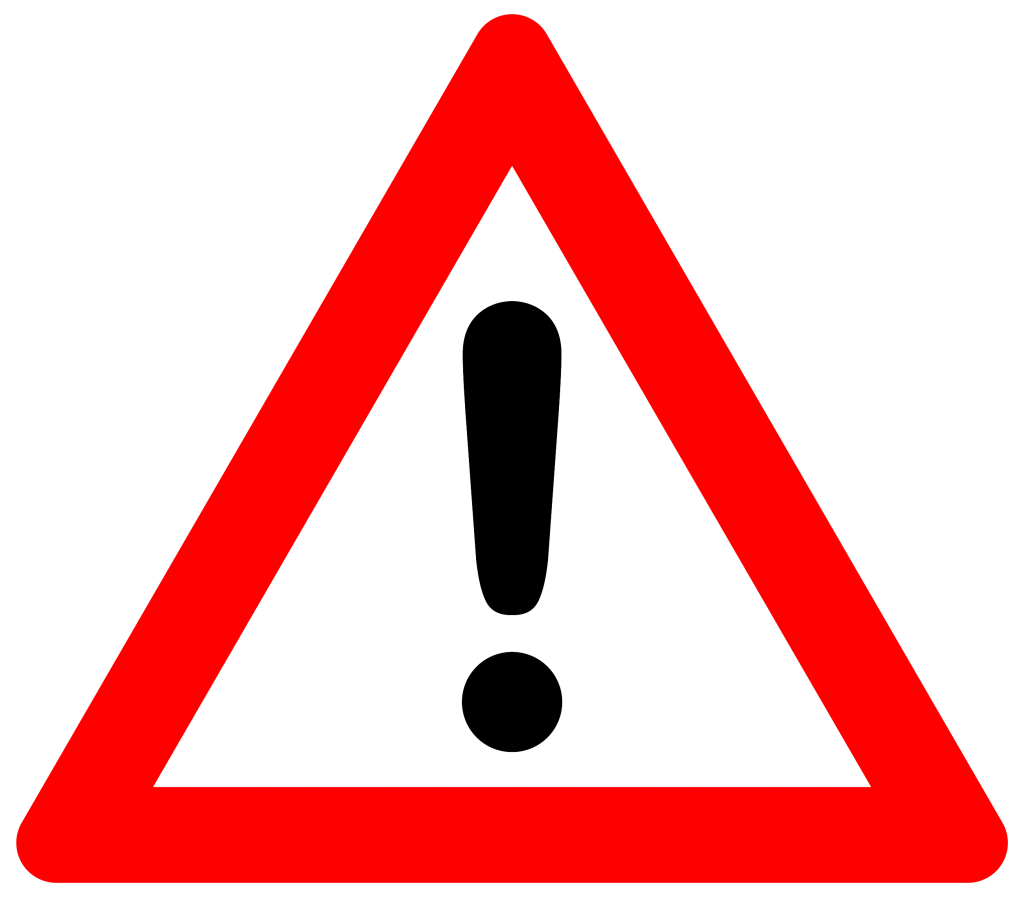
\includegraphics[scale=0.05]{Figures/triangle.png}
  \end{figure}
\end{flushright}

L'interesse non è mai nel comportamento in sé ma nel \textbf{costrutto}
misurato da quel comportamento. \pause

\emph{Costrutto}: un concetto psicologico non osservabile
\end{frame}

\begin{frame}{Cosa sono i test}
\phantomsection\label{cosa-sono-i-test-1}
I test cognitivi/neuropsicologi utilizzati in forense, sono test di
performance massima (o prestazione massima)

\begin{flushright}
  \emph{(Cronbach, 1990)}
\end{flushright}
\pause
\vspace{2em}

Essi presentano alcune caratteristiche (che discuteremo nel corso). Sono
diversi da questionari o test di \emph{risposta tipica}. \pause
\vspace{2em}

\begin{center}
La maggior parte dei test a cui ci faremo riferimento sono quelli di performance massima perché ritenuti più rilevanti recentemente nella valutazione forense
\end{center}
\end{frame}

\begin{frame}{Cosa sono i test}
\phantomsection\label{cosa-sono-i-test-2}
\begin{center}
  \textbf{Esempio:}
\end{center}
\vspace{2em}

\emph{Consideriamo il test Linguaggio Figurato 1.}

\emph{Il paziente un punteggio finale di 10.}

\emph{Cosa indica questo numero?} \pause \vspace{2em}

Il comportamento è l'\emph{indicatore di un costrutto} (con costrutto
indico genericamente un concetto psicologico non direttamente
osservabile)
\end{frame}

\begin{frame}{Cosa sono i test}
\phantomsection\label{cosa-sono-i-test-3}
\begin{figure}
  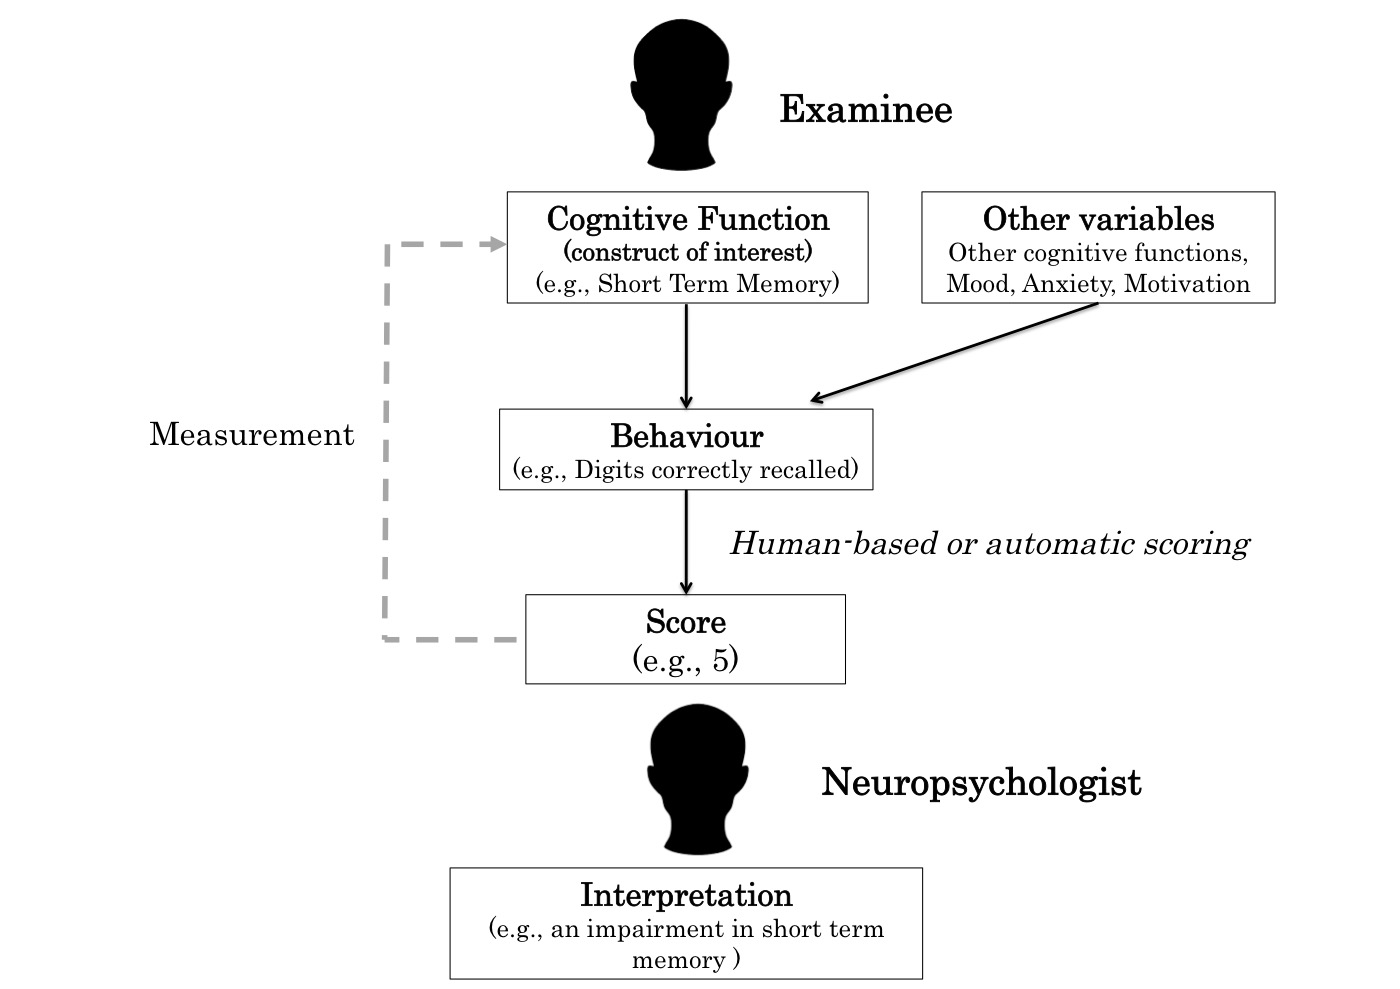
\includegraphics[scale=0.3]{Figures/measurement_diagramma.png}
\end{figure}

\begin{flushright}
  (Da Mondini, Cappelletti, Arcara, 2022)
\end{flushright}

\textbf{Costrutto}: Concetto psicologico non osservabile direttamente
\end{frame}

\begin{frame}{Cosa sono i test}
\phantomsection\label{cosa-sono-i-test-4}
Un esempio di test. Rivediamo l'esempio di Linguaggio Figurato 1
\end{frame}

\begin{frame}{Teoria dei test}
\phantomsection\label{teoria-dei-test}
\begin{center}
  \textbf{Classical Test Theory}
\end{center}

La \textbf{Teoria Classica dei test (Classical Test Theory, CTT)} È un
insieme di concetti di teoria di psicometria legati allo sviluppo di
test psicologici. Spesso si basa su principi di misurazione come quello
di Stevens \pause

Fanno parte della CTT, concetti come Validità e Affidabilità. \pause

La maggior parte dei test neuropsicologici (clinici e forensi),
implicitamente o esplicitamente utilizzano principi e assunti di CTT.
\pause

\href{https://en.wikipedia.org/wiki/Classical_test_theory}{\ul{https://en.wikipedia.org/wiki/Classical\_test\_theory}}
\end{frame}

\begin{frame}{Teoria dei test}
\phantomsection\label{teoria-dei-test-1}
\begin{center}
  \textbf{Classical Test Theory}
\end{center}

Il principio cardine della CTT è la seguente formula:

\begin{center}
$X = T + E$
\end{center}
\pause

\(X\) = punteggio osservato

\(T\) = punteggio vero

\(E\) = errore \pause \vspace{1.5em}

L'errore è indipendente dal punteggio vero.
\end{frame}

\begin{frame}{Teoria dei test}
\phantomsection\label{teoria-dei-test-2}
\begin{center}
  \textbf{I Limiti della Classical Test Theory}
\end{center}

La Teoria classica dei test ha dei problemi intrinseci. Ne citiamo
alcuni: \pause

\begin{itemize}[<+->]
\item
  Abilità del soggetto e complessità/difficoltà del test sono confuse
\item
  Errore e punteggio vero non sono spesso realmente indipendenti
\item
  Problemi nella definizione di forme parallele (studieremo questo
  quando vedremo cambiamenti nel tempo)
\end{itemize}

\emph{Consideriamo il possibile errore in un punteggio di Linguaggio
Figurato 1 pari a 8, 0, oppure di 15. L'errore è veramente indipendente
dal punteggio vero?}
\end{frame}

\begin{frame}{Teoria dei test}
\phantomsection\label{teoria-dei-test-3}
\begin{center}
  \textbf{Esempio script CTT}
\end{center}

Vedi esempio da link
\end{frame}

\begin{frame}{Teoria dei test}
\phantomsection\label{teoria-dei-test-4}
\begin{center}
  \textbf{Item Response Theory}
\end{center}

La Item Response Theory è una famiglia di metodi più avanzati che
cercano di modellare in maniera indipendente la difficoltà del task e le
abilità del soggetto.

Tra I modelli di IRT I più famosi (storicamente) sono I modelli di
Rasch, che permettono I modellare test in cui gli item hanno risposta
sì/no. \pause

I modelli di IRT hanno un'importante assunzione che spesso è critica per
test neuropsicologici e cioè l'unidimensionalità del costrutto. \pause

Si assume che il costrutto misurato dal test sia rappresentabile lungo
un'unica dimensione (non sia la combinazione di più costrutti).
\end{frame}

\begin{frame}{Teoria dei test}
\phantomsection\label{teoria-dei-test-5}
\begin{center}
  \textbf{Item Response Theory}
\end{center}

Esempio formula Modelli di Rasch (la cito per completezza): \vspace{2em}

\begin{figure}
  
\includegraphics[width=0.8\textwidth]{Figures/Rasch.png}
\end{figure}
\vspace{2em}

\href{https://www.publichealth.columbia.edu/research/population-health-methods/item-response-theory}{\ul{https://www.publichealth.columbia.edu/research/population-health-methods/item-response-theory}}
\end{frame}

\begin{frame}{Teoria dei test}
\phantomsection\label{teoria-dei-test-6}
\begin{center}
  \textbf{Item Response Theory – Rasch models}
\end{center}

\begin{figure}
  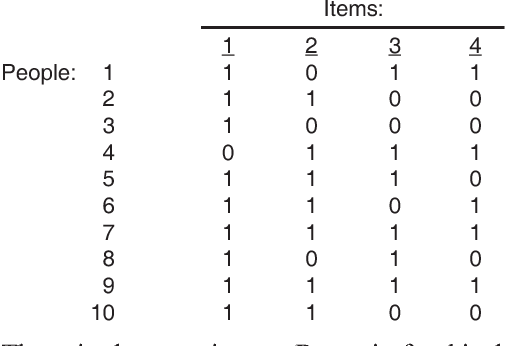
\includegraphics[width=0.7\textwidth]{Figures/Rasch_matrix.png}
\end{figure}

Per costruire modelli di Rasch/IRT si parte spesso da matrici di questo
tipo.
\end{frame}

\begin{frame}{Teoria dei test}
\phantomsection\label{teoria-dei-test-7}
\begin{center}
  \textbf{Classical Test Theory vs Item Response Theory}
\end{center}
\vspace{2em}

Sebbene I modelli di IRT siano psicometricamente più rigorosi, in questo
corso parlerò praticamente sempre di CTT perché la quasi totalità. Di
test disponibili per Neuropsicologia Clinica e forense sono sviluppati
secondo questo principio (e non con IRT).
\end{frame}

\begin{frame}{Teoria dei test}
\phantomsection\label{teoria-dei-test-8}
\begin{center}
  \textbf{Classical Test Theory vs Item Response Theory}
\end{center}

\emph{Perché non ci sono test sviluppati IRT, se sono più rigorosi?}
\pause

Un misto di aspetti teorici e praticità \pause

\begin{itemize}[<+->]
\tightlist
\item
  Sviluppare test con IRT è più costoso (e può andare più facilmente
  male)
\item
  spesso I costrutti neuropsiclologici per forense violano quasi per
  definizione l'unidimensionalità.
\item
  talvolta ad una diversa procedura, comunque IRT e CTT possono portare
  a risultati molto simili
  (\href{https://doi.org/10.1044/1092-4388(2006/003)}{Hula et al.,
  2006})
\end{itemize}
\end{frame}

\begin{frame}{Teoria dei test}
\phantomsection\label{teoria-dei-test-9}
\begin{center}
  \textbf{Classical Test Theory vs Item Response Theory}
\end{center}

L'assunto di undimensionalità, assume che:

\begin{itemize}[<*>] 
\item gli Item possano essere ordinati secondo la loro difficoltà e che
\item la probabilità di rispondere correttamente ad un Item rifletta (più o meno) alla sua difficoltà: più un item è difficile meno probabile è rispondere correttamente.
\end{itemize}

Questo è facile pensarlo per test che includano item in cui è facile
gradare la difficoltà (es. esercizi di matematica), ma con un test
neuropsicologico?
\end{frame}

\begin{frame}{Teoria dei test}
\phantomsection\label{teoria-dei-test-10}
\begin{center}
  \textbf{Classical Test Theory vs Item Response Theory}
\end{center}
\vspace{2em}

\begin{columns}
  \begin{column}{0.5\textwidth}
    \begin{figure}
    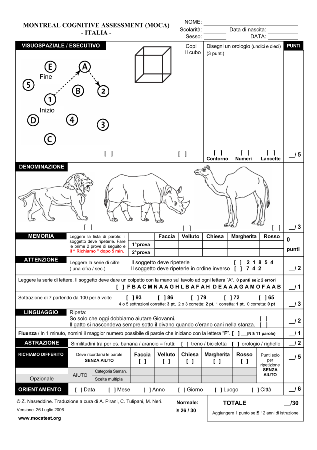
\includegraphics[scale=0.5]{Figures/MOCA.png}
    \end{figure}
  \end{column}
  \begin{column}{0.5\textwidth}
    È facile gradare gli item del moca per difficoltà?
  \end{column}
\end{columns}
\end{frame}

\begin{frame}{Teoria dei test}
\phantomsection\label{teoria-dei-test-11}
\begin{center}
  \textbf{Classical Test Theory vs Item Response Theory}
\end{center}
\vspace{1.5em}

\begin{figure}
  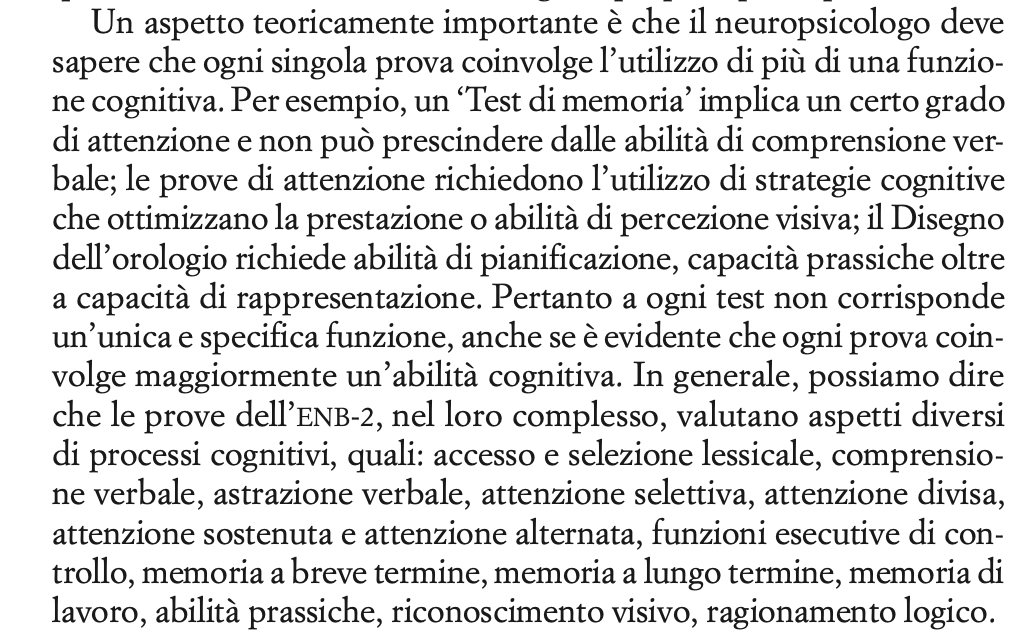
\includegraphics[scale=0.5]{Figures/ENB2_cit.png}
\end{figure}

\footnotesize
\begin{flushright}
  \textit{da ENB-2 p. 25, Mondini et al. 2011}
\end{flushright}
\end{frame}

\begin{frame}{Costrutti}
\phantomsection\label{costrutti}
\begin{center}
  \textbf{I costrutti misurati tramite i test neuropsicologici}
\end{center}

\textbf{Costrutto}: Concetto psicologico non osservabile direttamente

\emph{Quali sono i tipici costrutti misurati dai test neuropsicologici?}

\begin{figure}
  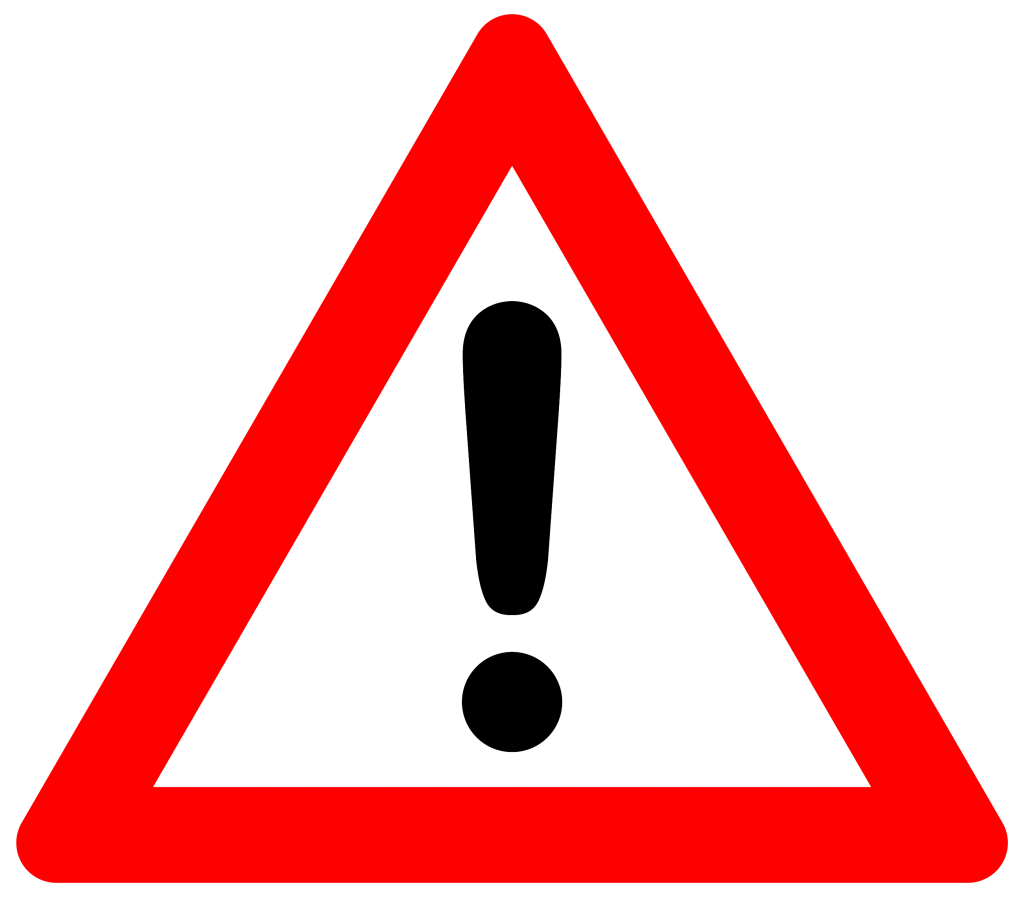
\includegraphics[scale=0.05]{Figures/triangle.png}
\end{figure}

I test neuropsicologici misurano costrutti di diverso tipo
\end{frame}

\begin{frame}{Costrutti}
\phantomsection\label{costrutti-1}
\begin{center}
  \textbf{fI costrutti misurati tramite i test neuropsicologici sono a diversi livelli}
  \vspace{2em}

  Abilità funzionali
  
  {\small Costrutti più generici}
  
  {\footnotesize Funzioni cognitive}
\end{center}
\end{frame}

\begin{frame}{Costrutti}
\phantomsection\label{costrutti-2}
\begin{center}
  \textbf{1) I test neuropsicologici misurano funzioni cognitive}
\end{center}
\vspace{2em}

Esempi

Il digit span misura la (capacità della) memoria a breve termine.

Il test di memoria con interferenza (ENB-3) misura la (capacità della)
memoria di lavoro.

Il TMT-A misura la (capacità di) ricerca visuo-spaziale, di attenzione
selettiva e di velocità psicomotoria.

\begin{flushright}
  \textit{da ENB-3 (Mondini et al., 2011)}
\end{flushright}
\end{frame}

\begin{frame}{Costrutti}
\phantomsection\label{costrutti-3}
\begin{center}
  \textbf{2) I test neuropsicologici misurano costrutti più generici}
\end{center}
\vspace{2em}

Esempi

Il Fab-it (Appollonio et al., 2005) misura il generale stato delle
funzioni esecutive

Il SET (Dodich et al., 2015), nel punteggio globale misura l'abilità di
teoria della mente.

Linguaggio Figurato 1 in APACS (Arcara \& Bambini, 2016), il punteggio
indica la capacità di andare oltre il significato letterale e di
comprendere il linguaggio figurato.
\end{frame}

\begin{frame}{Costrutti}
\phantomsection\label{costrutti-4}
\begin{center}
  \textbf{2) I test neuropsicologici misurano costrutti più generici}
\end{center}
\vspace{2em}

Esempi

Driving Scenes Test (Brown et al., 2005)

NADL-F (Arcara et al., 2017)
\href{https://osf.io/d9jng/}{\ul{https://osf.io/d9jng/}} \vspace{2em}

\emph{I test ecologici molto utili per risposte concrete sulla vita
quotidiana ma possono essere lunghi o poco disponibili}
\end{frame}

\begin{frame}{Costrutti}
\phantomsection\label{costrutti-5}
\begin{center}
  \textbf{I costrutti misurati tramite i test neuropsicologici sono a diversi livelli}
  \vspace{2em}

  Abilità funzionali
  (es. Abilità di guida) 
  
  {\small Costrutti più generici
  (es. Efficienza funzioni esecutive)}
  
  {\footnotesize Funzioni cognitive
  (es. Memoria di lavoro)}
  
\end{center}
\end{frame}

\begin{frame}{Costrutti}
\phantomsection\label{costrutti-6}
\begin{center}
  \textbf{I costrutti misurati tramite i test neuropsicologici sono a diversi livelli}
\end{center}
\vspace{2em}

Il fatto che I costrutti siano a gerarchie diverse implica che il
costrutto misurato da un test potrebbe essere incluso all'interno di un
costrutto misurato da un altro test

Questo aspetto verrà ripreso nel punto in cui discuteremo
dell'interpretazione dei test.
\end{frame}

\begin{frame}{Altre tipologie di test}
\phantomsection\label{altre-tipologie-di-test}
I test neuropsicologici sono il più delle volte test di performance
massima cioè test in cui al soggetto è chiesto di fare il meglio
possibile.

Talvolta vengono usate anche scale funzionali o questionari (non di
prestazione massima).

La \textbf{IADL} (Lawton \& Brody, 1970) è una scala dell'autonomia
nella vita quotidiana, non è un vero e proprio test.

Il \textbf{COAST} (Bambini et al., 2016) è una scala per la valutazione
dell'efficacia comunicativa dal punto di vista del paziente o del
caregiver.

Test di personalità, di umore, etc. \textbf{NON} sono test di
prestazione massima
\end{frame}

\begin{frame}{Riflessione su misurazione di specifici costrutti}
\phantomsection\label{riflessione-su-misurazione-di-specifici-costrutti}
\textbf{Perché è utile misurare un certo costrutto?} \pause

Talvolta ci si dimentica il \emph{perché} si vuole misurare un certo
costrutto e perché potrebbe essere utile, sia a livello clinico, sia a
livello forense. \pause

C'è spesso un'assunzione di fondo: che la valutazione di aspetti
cognitivi (anche di base) ci può dire qualcosa su come funziona
quotidianamente una persona e quindi darci informazioni sul suo
comportamento in situazioni al di fuori della valutazione

Si assume che ci sia una \textbf{validità
ecologica}\footnote<.->[frame]{La validità ecologica verrà trattata
  nelle slides 4 Validità e Affidabilità} di uno specifico test (il
fatto che sia andato male in questo test implica che nella vita
quotidiana c'è un effetto, che ha rilevanza per il mio caso forense)
\end{frame}

\begin{frame}{Riflessione su misurazione di specifici costrutti}
\phantomsection\label{riflessione-su-misurazione-di-specifici-costrutti-1}
Assumere che i risultati del test ci dicano qualcosa sulla vita
quotidiana non è sbagliato in sé, ma non dimentichiamo che (a meno che
di validità ecologica comprovata da dati scientifici) questa è
un'interpretazione.
\end{frame}

\begin{frame}{Recap}
\phantomsection\label{recap}
\begin{figure}
  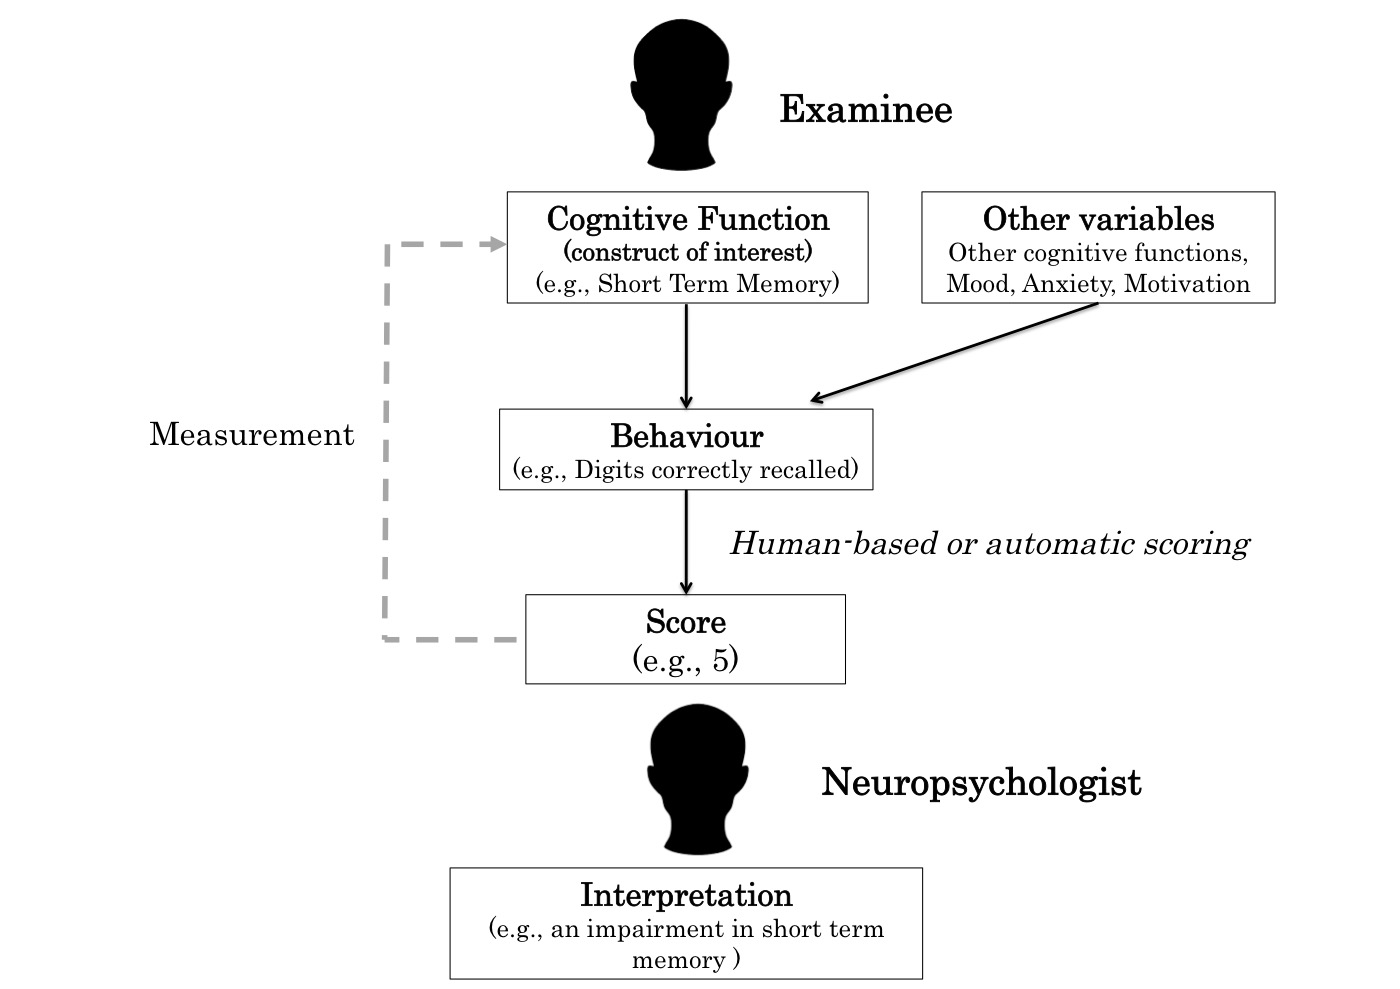
\includegraphics[scale=0.3]{Figures/measurement_diagramma.png}
\end{figure}

\begin{flushright}
  (Da Mondini, Cappelletti, Arcara, 2022)
\end{flushright}

\textbf{Costrutto}: Concetto psicologico non osservabile direttamente
\end{frame}




\end{document}
